\documentclass[authoryear,preprint]{sigplanconf}
\usepackage{amsmath}
\usepackage{listings} 
\usepackage{stmaryrd}
\usepackage{latexsym}
\usepackage{amssymb}
\usepackage{xcolor}
\usepackage{courier}
\usepackage{thmtools}
\usepackage{bbold}
\usepackage{tikz}
\usepackage{proof}
\usepackage{graphicx}

\newcommand{\bdim}[1]{\textsf{dim}(#1)}
\newcommand{\Rule}[4]{
\makebox{{\rm #1}
$\displaystyle
\frac{\begin{array}{l}#2\\\end{array}}
{\begin{array}{l}#3\\\end{array}}$
 #4}}
\newcommand{\proves}{\vdash}
\newcommand{\symc}[1]{\mathit{sym}~#1}
\newcommand{\jdg}[3]{#2 \proves_{#1} #3}
\newcommand{\adjoint}[1]{#1^{\dagger}}
\newcommand{\iso}{\leftrightarrow}
\newcommand{\identlp}{\mathit{identl}_+}
\newcommand{\identrp}{\mathit{identr}_+}
\newcommand{\swapp}{\mathit{swap}_+}
\newcommand{\assoclp}{\mathit{assocl}_+}
\newcommand{\assocrp}{\mathit{assocr}_+}
\newcommand{\identlt}{\mathit{identl}_*}
\newcommand{\identrt}{\mathit{identr}_*}
\newcommand{\swapt}{\mathit{swap}_*}
\newcommand{\assoclt}{\mathit{assocl}_*}
\newcommand{\assocrt}{\mathit{assocr}_*}
\newcommand{\distz}{\mathit{dist}_0}
\newcommand{\factorz}{\mathit{factor}_0}
\newcommand{\dist}{\mathit{dist}}
\newcommand{\factor}{\mathit{factor}}
\newcommand{\idc}{\mathit{id}}
\newcommand{\plus}{\raisebox{.4\height}{\scalebox{.6}{+}}}
\newcommand{\minus}{\raisebox{.4\height}{\scalebox{.8}{-}}}
\newcommand{\mm}{\texttt{-}}
\newcommand{\pp}{\texttt{+}}
\newcommand{\negp}[1]{\textit{neg}(#1)}
\newcommand{\inl}[1]{\textsf{inl}~#1}
\newcommand{\inr}[1]{\textsf{inr}~#1}
\newcommand{\lolli}{\multimap} 
\newcommand{\cubt}{\mathbb{T}}
\newcommand{\den}[1]{\llbracket #1 \rrbracket}
\newcommand{\denc}[1]{\llbracket #1 \rrbracket^c}
\newcommand{\nodet}[2]{\fcolorbox{black}{white}{$#1$}\fcolorbox{black}{gray!20}{$#2$}}

\begin{document}
\special{papersize=8.5in,11in}
\setlength{\pdfpageheight}{\paperheight}
\setlength{\pdfpagewidth}{\paperwidth}

\newcommand{\alt}{~|~}
\lstnewenvironment{code}{\lstset{basicstyle={\sffamily\footnotesize}}}{}

\lstset{frame=none,
         language=Haskell,
         basicstyle=\sffamily, 
         numberstyle=\tiny,
         numbersep=5pt,
         tabsize=2,    
         extendedchars=true,
         breaklines=true,   
         breakautoindent=true,
         keywordstyle=\color{black},
         captionpos=b,
         stringstyle=\color{black}\ttfamily,
         showspaces=false,  
         showtabs=false,    
         framexleftmargin=2em,
         framexbottommargin=1ex,
         showstringspaces=false
         basicstyle=\sffamily,
         columns=[l]flexible,
         flexiblecolumns=true,
         aboveskip=\smallskipamount,
         belowskip=\smallskipamount,
         lineskip=-1pt,
         xleftmargin=1em,
         escapeinside={/+}{+/},
         keywords=[1]{Monad,Just,Nothing,type,data,right,left,id,where,do,
                     if,then,else,let,in},
         literate=
           {+}{{$\;+\;$}}1 
           {/}{{$/$}}1 
           {*}{{$\;*\;$}}1
           {=}{{$=\ $}}1 
           {/=}{{$\not=$}}1
           {[]}{$[\;]$}2
           {<}{{$<$}}1 
           {>}{{$>$}}1 
           {++}{{$+\!\!\!+\;$}}1 
           {::}{{$:\mkern -2.5mu:\;$}}1
           {&&}{{$\&\!\!\!\&$}}2
           {:=:}{{$:\mkern -2mu=\mkern -2mu:\;$}}3
           {:+:}{{$:\mkern -5mu+\mkern -5mu:\;$}}3
           {:-:}{{$:\mkern -5mu-\mkern -5mu:\;$}}3
           {:*:}{{$:\mkern -5mu*\mkern -5mu:\;$}}3
           {$}{{\texttt{\$}\hspace{0.5em}}}1
           {`}{$^\backprime$}1
           {==}{{$=\!=\;$}}2
           {===}{{$\equiv\;$}}2
           {->}{{$\rightarrow\;$}}2 
           {>=}{{$\geq$}}2 
           {<=}{{$\leq$}}2 
           {>=0}{{$\geq_\zerog\;$}}2 
           {<=0}{{$\leq_\zerog\;$}}2 
           {==0}{{$=_\zerog\;$}}2 
           {>0}{{$>_\zerog\;$}}2 
           {<0}{{$<_\zerog\;$}}2 
           {<-}{{$\leftarrow$}}2
           {=>}{{$\Rightarrow\;$}}2
           {<<}{{$\ll$}}2 
           {>>}{{$\gg\;$}}2
           {>>>}{{$\ggg\;$}}3 
           {<<<}{{$\lll\;$}}3
           {>>=}{{$\gg\mkern -2.5mu=\;$}}3
           {=<<}{{$=\mkern -2.5mu\ll\;$}}3
           {<|}{$\lhd\;$}2
           {<||}{$\unlhd\;$}2
           {\ ||\ }{$\|$}1
           {\\}{$\lambda$}1
           {:>}{{$\rhd$}}2
           {||>}{{$\unrhd$}}2
           {_}{{$\_$}}1
           {_B}{{$_b$}}2
           {forall}{{$\forall$}}1
}

\lstset{postbreak=\raisebox{0ex}[0ex][0ex]
        {\ensuremath{\hookrightarrow}}}
\lstset{breaklines=true, breakatwhitespace=true}
\lstset{numbers=none, numbersep=5pt, stepnumber=2, numberstyle=\scriptsize}
\lstset{rangeprefix=/*!\ , rangesuffix=\ !*\/, includerangemarker=false}

%% double-blind reviewing...
\title{Cubical Polarized Types}
\authorinfo{}{}{}
\maketitle

\begin{abstract}
\ldots
\end{abstract}

%%%%%%%%%%%%%%%%%%%%%%%%%%%%%%%%%%%%%%%%%%%%%%%%%%%%%%%%%%%%%%%%%%%%%%%%%%%%%%
\section{Introduction}

The \textbf{Int} construction or the $\mathcal{G}$ construction are neat. As
Neel K. explains, given first-order types and feedback you get higher-order
functions. But if you do the construction on the additive structure, you lose
the multiplicative structure. It turns out that this is related to a deep
open problem in algebraic topology and homotopy theory that was recently
solved. We ``translate'' that solution to a computational type-theoretic
world. This has evident connections to homotopy (type?) theory that remain to
be investigated.

%%%%%%%%%%%%%%%%%%%%%%%%%%%%%%%%%%%%%%%%%%%%%%%%%%%%%%%%%%%%%%%%%%%%%%%%%%%%%%
\section{The \textbf{Int} Construction} 

Explain in detail perhaps with Haskell embedding and type functions etc. The
key insight it to add ``negative'' types representing demand for values. This
is how you get functions.

%%%%%%%%%%%%%%%%%%%%%%%%%%%%%%%%%%%%%%%%%%%%%%%%%%%%%%%%%%%%%%%%%%%%%%%%%%%%%%
\section{The Problem and the Intuitive Solution}

We lose the multiplicative structure. No evident way to define the
multiplication functor. Perhaps there is a clever way. But this turns out to
be a well-known open problem. Review the problem and tell the story from the
algebraic topology perspective. Regular first-order types are viewed as
$0$-dimensional cubes. Generalize to $n$-dimensional cubes.

%%%%%%%%%%%%%%%%%%%%%%%%%%%%%%%%%%%%%%%%%%%%%%%%%%%%%%%%%%%%%%%%%%%%%%%%%%%%%%
\section{The Type Structure}

We first define the syntax a semantic model of types and then discuss type
isomorphisms.

%%%%%%%%%%%%%%%%%%%%
\subsection{Negative and Cubical Types}

We use $t$ for regular first-order types which include the empty type, the
unit type, and conventional sum and product types. We call these types
$0$-dimensional. We use $\tau$ for cubical types of dimension 1 or higher:
these have the same syntactic structure as regular types except that they
also include \emph{negative} types. The syntax of the types is summarized
below:
\[\begin{array}{lrcl}
\textit{types of dimension $0$} & 
  t &::=& 0 \alt 1 \alt t_1 + t_2 \alt t_1 * t_2 \\
\textit{types of dimensions $\geq 1$} & 
  \tau &::=& \Box t \alt \tau_1 + \tau_2 \alt \tau_1 * \tau_2 \alt - \tau
\end{array}\]
We use $\tau_1 - \tau_2$ to abbreviate $\tau_1 + (- \tau_2)$ and more
interestingly $\tau_1 \lolli \tau_2$ to abbreviate $(- \tau_1) + \tau_2$.
The $\Box$ is used to make explicit the injection of a first-order type into
a 1-dimensional type. We omit the explicit injection when
convenient. Formally, the \emph{dimension} of a type is defined as follows:
\[\begin{array}{rcl}
\bdim{t} &=& 0 \\
\bdim{\Box t} &=& 1 \\
\bdim{\tau_1 + \tau_2} &=& \max(\bdim{\tau_1},\bdim{\tau_2}) \\
\bdim{\tau_1 * \tau_2} &=& \bdim{\tau_1} + \bdim{\tau_2} \\
\bdim{- \tau} &=& \bdim{\tau}
\end{array}\]

It is easy to find a model for $0$-dimensional types: finite sets are such a
model. In more detail:
\[\begin{array}{rcl}
\den{0} &=& \emptyset \\
\den{1} &=& \{ \star \} \\
\den{t_1 + t_2} &=& \den{t_1} \uplus \den{t_2} \\
\den{t_1 * t_2} &=& \den{t_1} \times \den{t_2} 
\end{array}\]
The type 0 maps to the empty set. The type 1 maps to a singleton set. The sum
of types maps to disjoint union of sets. The product of types maps to the
cartesian product of sets. We usually use $S$ for the denotation of these
conventional first-order types. Note that our (simple) semantics of types
identifies several structurally different types such as $(1+(1+1))$ and
$((1+1)+1)$. In some sense, this is innocent as the types are
isomorphic. However, in the operational semantics discussed in the next
section, we make the computational content of such type isomorphisms
explicit.

For cubical types of dimension $n \geq 1$, their denotations, usually written
as $\cubt$, are $n$-dimensional ``polarized cubes.'' Such an $n$-dimensional
cube $\nodet{\cubt_1}{\cubt_2}$ consists of a positive subspace $\cubt_1$ and
a negative subspace $\cubt_2$ (shaded in gray). Each of the subspaces are
cubes of a lower dimension; the $0$-dimensional case reduces to the
denotation of conventional first-order types. As we explain below, cubical
sets are closed under sums, differences, products.

A 1-dimensional cube looks like $\nodet{S_1}{S_2}$ which intuitively
corresponds to the difference $t_1 - t_2$ (formally $\Box t_1 + (- \Box
t_2)$) of the two types whose denotations are $S_1$ and $S_2$ respectively. A
2-dimensional cube looks like
$\nodet{(\nodet{S_1}{S_2})}{(\nodet{S_3}{S_4})}$ which intuitively
corresponds to the iterated difference of the appropriate types
$(t_1-t_2)-(t_3-t_4)$ where the product of the successive signs from the
outermost box encodes the sign.

We now give the full denotation of cubical types:
\[\begin{array}{rcl}
\denc{\Box t} &=& \nodet{\den{t}}{\phantom{\den{t}}} \\
\denc{\tau_1 + \tau_2} &=& \denc{\tau_1} \oplus \denc{\tau_2} \\
\denc{\tau_1 * \tau_2} &=& \denc{\tau_1} \otimes \denc{\tau_2} \\
\denc{- \tau} &=& \ominus \denc{\tau}
\end{array}\]
where the operations $\oplus$, $\otimes$, and $\ominus$ are defined below.
It is possible, in general, for the binary trees representing the cubes not
be balanced. It is however always possible to embed an $n$-dimensional cube
into a cube of a larger dimension using the fact (to be justified using a
$\Pi$-combinator that witnesses this isomorphism in the next section) that
$t$ is equivalent to $t-0$ and to $(t-0)-0$ and so on, i.e.,
\[
S = \nodet{S}{\phantom{S}} = 
  \nodet{\nodet{S}{\phantom{S}}}
        {\phantom{{\nodet{S}{\phantom{S}}}}} = \ldots \\
\]
In the recursive definition of addition below, we assume that the smaller
cube has been extended to the dimension of the larger one: 
\[\begin{array}{rcl}
\ominus~S &=& \nodet{\phantom{S}}{S} \\
\ominus~\nodet{\cubt_1}{\cubt_2} &=& \nodet{\ominus~\cubt_2}{\ominus~\cubt_1} \\
\\
S_1 \oplus S_2 &=& S_1 \uplus S_2 \\
(\nodet{\cubt_1}{\cubt_2}) \oplus (\nodet{\cubt_3}{\cubt_4}) &=& 
  \nodet{\cubt_1 \oplus \cubt_3}{\cubt_2 \oplus \cubt_4} \\
\\
S_1 \otimes S_2 &=& S_1 \times S_2 \\
S \otimes (\nodet{\cubt_1}{\cubt_2}) &=& 
  \nodet{S \otimes \cubt_1}{S \otimes \cubt_2} \\
(\nodet{\cubt_1}{\cubt_2}) \otimes \cubt &=& 
  \nodet{\cubt_1 \otimes \cubt}{\cubt_2 \otimes \cubt}
\end{array}\]

\begin{figure*}
\[\begin{array}{c}
\nodet{S_1}{S_2}
\quad\otimes\quad
\nodet{(\nodet{S_3}{S_4})}{(\nodet{S_5}{S_6})} \quad= \\
\\
\nodet{(\nodet{{(\nodet{S_1 \times S_3}{S_1 \times S_4})}}
              {{(\nodet{S_1 \times S_5}{S_1 \times S_6})}})}
      {(\nodet{{(\nodet{S_2 \times S_3}{S_2 \times S_4})}}
              {{(\nodet{S_2 \times S_5}{S_2 \times S_6})}})}
\end{array}\]
\caption{\label{mult}Example of multiplication of two cubical sets.}
\end{figure*}

\noindent The definition of negation is natural: it recursively swaps the
positive and negative subspaces. We note that the general definitions of sums
and products reduce to the conventional sums and products for $0$-dimensional
types. Also the sum of 1-dimensional types reduces to the sum used in the
\textbf{Int} construction and that addition and negation do not increase the
dimensions. The interesting new development is the definition of
products. The example in Fig.~\ref{mult} illustrates a general pattern: the
product of an $n$-dimensional type with an $m$-dimensional type gives an
$(n+m)$-dimensional type. For low dimensions such as the ones used in the
example above, it is possible to visualize what is happening in coordinate
space (see Fig.~\ref{multv}).

\begin{figure*}
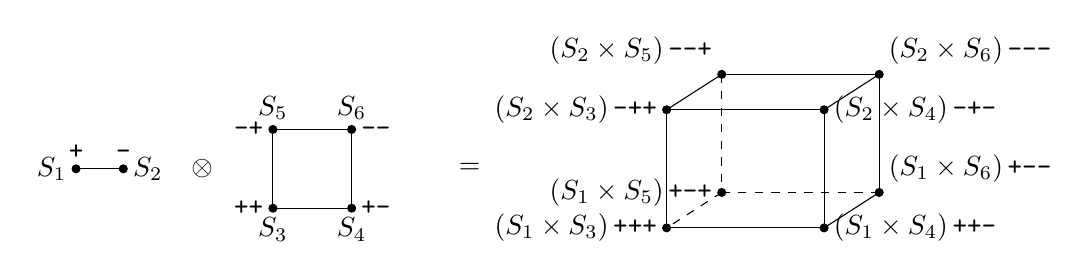
\begin{tikzpicture}
\node[above] at (0,0) {\pp};
\node[left] at (0,0) {$S_1$};
\draw[fill] (0,0) circle [radius=0.05];
\node[above] at (0.6,0) {\mm};
\node[right] at (0.6,0) {$S_2$};
\draw[fill] (0.6,0) circle [radius=0.05];
\draw[-] (0,0) -- (0.6,0);
\node at (1.6,0) {$\otimes$}; 

%%
\node[left] at (2.5,-0.5) {\pp\pp};
\node[below] at (2.5,-0.5) {$S_3$};
\draw[fill] (2.5,-0.5) circle [radius=0.05];
\node[right] at (3.5,-0.5) {\pp\mm};
\node[below] at (3.5,-0.5) {$S_4$};
\draw[fill] (3.5,-0.5) circle [radius=0.05];
\draw[-] (2.5,-0.5) -- (3.5,-0.5);
\draw[-] (2.5,-0.5) -- (2.5,0.5);
\node[left] at (2.5,0.5) {\mm\pp};
\node[above] at (2.5,0.5) {$S_5$};
\draw[fill] (2.5,0.5) circle [radius=0.05];
\node[right] at (3.5,0.5) {\mm\mm};
\node[above] at (3.5,0.5) {$S_6$};
\draw[fill] (3.5,0.5) circle [radius=0.05];
\draw[-] (2.5,0.5) -- (3.5,0.5);
\draw[-] (3.5,-0.5) -- (3.5,0.5);
%% 
\node at (5,0) {$=$};
%% 
\node[left] at (7.5,0.75) {$(S_2 \times S_3)$\,\mm\pp\pp};
\draw[fill] (7.5,0.75) circle [radius=0.05];
\node[right] at (9.5,0.75) {$(S_2 \times S_4)$\,\mm\pp\mm};
\draw[fill] (9.5,0.75) circle [radius=0.05];
\node[above right] at (10.2,1.2) {$(S_2 \times S_6)$\,\mm\mm\mm};
\draw[fill] (10.2,1.2) circle [radius=0.05];
\node[above left] at (8.2,1.2) {$(S_2 \times S_5)$\,\mm\mm\pp};
\draw[fill] (8.2,1.2) circle [radius=0.05];
%%
\node[left] at (7.5,-0.75) {$(S_1 \times S_3)$\,\pp\pp\pp};
\draw[fill] (7.5,-0.75) circle [radius=0.05];
\node[right] at (9.5,-0.75) {$(S_1 \times S_4)$\,\pp\pp\mm};
\draw[fill] (9.5,-0.75) circle [radius=0.05];
\node[above right] at (10.2,-0.3) {$(S_1 \times S_6)$\,\pp\mm\mm};
\draw[fill] (10.2,-0.3) circle [radius=0.05];
\node[left] at (8.2,-0.3) {$(S_1 \times S_5)$\,\pp\mm\pp};
\draw[fill] (8.2,-0.3) circle [radius=0.05];
%%
\draw[-] (7.5,0.75) -- (9.5,0.75);
\draw[-] (9.5,0.75) -- (10.2,1.2);
\draw[-] (10.2,1.2) -- (8.2,1.2);
\draw[-] (8.2,1.2) -- (7.5,0.75);
%%
\draw[-] (7.5,-0.75) -- (9.5,-0.75);
\draw[-] (9.5,-0.75) -- (10.2,-0.3);
\draw[-,dashed] (10.2,-0.3) -- (8.2,-0.3);
\draw[-,dashed] (8.2,-0.3) -- (7.5,-0.75);
%%
\draw[-] (7.5,0.75) -- (7.5,-0.75);
\draw[-] (9.5,0.75) -- (9.5,-0.75);
\draw[-] (10.2,1.2) -- (10.2,-0.3);
\draw[-,dashed] (8.2,1.2) -- (8.2,-0.3);
\end{tikzpicture}
\caption{\label{multv}Visualization of multiplication of two cubical sets.}
\end{figure*}

%%%%%%%%%%%%%%%%%%%%
\subsection{Type Isomorphisms}

\begin{verbatim}
To complete the story we need to 
define morphisms. (More on this below.)
Once we have a notion of morphism we 
can check whether X + 0 is the same
as X etc. i.e., we can check all the 
ring equivalences. 

Ok so what are the morphisms between 
these cubical objects? We know what
they are for 1-dimensional cubes: 
they are the pi combinabors. We also
know what they are for the 2-dimensional 
cubes: a maps (A-B) ==> (C-D) 
is a Pi map between A+D <=> C+B. 
How to generalize this? 

Why is there no trace in the ring 
completion paper??? What are 
the morphisms in that paper?

The ring completion paper produces
a simplicial category.

p. 3 talks about the group cancellation
as subcubes along the diagonal... 

We shouldn't focus on denotations. We want
an operational semantics for pi with 
negatives. The same way that Neel turned
the G construction into code that does
something neat; we want to turn that 
ring completion construction into code
that produces h.o. functions without
losing the multiplicative structure.

Show how to embed a square in 2D into
each of the faces of the 3D cube.

1D into 2D:

(a-b) => (a-b)-(0-0)
(a-b) => (a-0)-(b-0)
(a-b) => (0-b)-(0-a)
(a-b) => (0-0)-(b-a)

\end{verbatim}

%%%%%%%%%%%%%%%%%%%%%%%%%%%%%%%%%%%%%%%%%%%%%%%%%%%%%%%%%%%%%%%%%%%%%%%%%%%%%%
\section{A Reversible Language with Cubical Types} 

We first define values then combinators that manipulate the values to witness
the type isomorphisms.

%%%%%%%%%%%%%%%%%%
\subsection{Values} 

Now that the type structure is defined, we turn our attention to the notion
of values. For conventional first-order types, the values are also
conventional:
\[
\infer{() : 1}{} 
\qquad
\infer{\inl{v} : t_1 + t_2}{v : t_1}
\qquad
\infer{\inr{v} : t_1 + t_2}{v : t_2}
\qquad
\infer{(v_1,v_2) : t_1 * t_2}{v_1 : t_1 & v_2 : t_2}
\]
For cubical types, the values are more involved. Intuitively, a value of the
$n$-dimensional type $\tau$ is an element of one of the sets located in a
corner of the $n$-dimensional cube denoted by $\tau$. Thus to specify a
value, we must specify one of the corners of the cube which can easily be
done using a sequence $p$ of $+$ and $-$ polarities indicating how to
navigate the cube in each successive dimension starting from a fixed origin
to reach the desired corner. We denote such values as $v^{p}$ and use
$\epsilon$ for the empty sequence of polarities. One can think of the
sequence of signs as denoting a path in the binary tree representation of
cubical types. Formally:
\[\begin{array}{c}
\infer[\textit{base}]{v^{+} : t}{v : t} \\
\\
\infer[\textit{left}]{(\inl{v})^{p} : \tau_1 + \tau_2}{v^{p} : \tau_1}
\qquad
\infer[\textit{right}]{(\inr{v})^{p} : \tau_1 + \tau_2}{v^{p} : \tau_2} \\
\\
\infer[\textit{prod}]{(v_1,v_2)^{p_1 \cdot p_2} : \tau_1 * \tau_2}
      {v_1^{p_1} : \tau_1 & v_2^{p_2} : \tau_2} \\
\\
\infer[\textit{neg}]{v^{\negp{p}} : - \tau}{v^p : \tau} 
\end{array}\]
The rule \textit{base} states that a conventional first-order value can be
viewed as trivial $0$-dimensional cubical value. The rules \textit{left} and
\textit{right} reflect the fact that sums do not increase the dimension and
works pointwise. The rule \textit{prod} is the most involved one: it
increases the dimension by \emph{concatenating} the two dimensions in its
arguments. For example, if we pair $v_1^{\pp}$ and $v_2^{\mm\pp}$ we get
$(v_1,v_2)^{\pp\mm\pp}$. The rule \textit{neg} shows that a negative value
$v$ is located at the ``opposite'' corner of $v$ which is calculated as
follows:
\[\begin{array}{rcl}
\negp{\epsilon} &=& \epsilon \\
\negp{+p} &=& -\negp{p} \\
\negp{-p} &=& +\negp{p}
\end{array}\]

%%%%%%%%%%%%%%%%%%
\subsection{Combinators} 

The terms of $\Pi$ witness type isomorphisms of the form $b \iso b$. They
consist of base isomorphisms, as defined below, and their composition.
\[\begin{array}{rrcll}
\identlp :&  0 + b & \iso & b &: \identrp \\
\swapp :&  b_1 + b_2 & \iso & b_2 + b_1 &: \swapp \\
\assoclp :&  b_1 + (b_2 + b_3) & \iso & (b_1 + b_2) + b_3 &: \assocrp \\
\identlt :&  1 * b & \iso & b &: \identrt \\
\swapt :&  b_1 * b_2 & \iso & b_2 * b_1 &: \swapt \\
\assoclt :&  b_1 * (b_2 * b_3) & \iso & (b_1 * b_2) * b_3 &: \assocrt \\
\distz :&~ 0 * b & \iso & 0 &: \factorz \\
\dist :&~ (b_1 + b_2) * b_3 & \iso & (b_1 * b_3) + (b_2 * b_3)~ &: \factor
\end{array}\]
Each line of the above table introduces a pair of dual
constants\footnote{where $\swapp$ and $\swapt$ are self-dual.} that witness
the type isomorphism in the middle.  These are the base (non-reducible) terms
of the second, principal level of $\Pi$. Note how the above has two readings:
first as a set of typing relations for a set of constants. Second, if these
axioms are seen as universally quantified, orientable statements, they also
induce transformations of the (traditional) values. The (categorical or
homotopical) intuition here is that these axioms have computational content
because they witness isomorphisms rather than merely stating an extensional
equality.

The isomorphisms are extended to form a congruence relation by adding the
following constructors that witness equivalence and compatible closure:

\begin{table}[t]
\hrule\medskip
\begin{center} 
\Rule{}
{}
{\jdg{}{}{\idc : b \iso b}}
{}
\quad 
\Rule{}
{\jdg{}{}{c : b_1 \iso b_2}}
{\jdg{}{}{\symc{c} : b_2 \iso b_1}}
{}
\quad
\Rule{}
{\jdg{}{}{c_1 : b_1 \iso b_2} \quad c_2 : b_2 \iso b_3}
{\jdg{}{}{c_1 \fatsemi c_2 : b_1 \iso b_3}}
{}
\\ \bigskip
\Rule{}
{\jdg{}{}{c_1 : b_1 \iso b_2} \quad c_2 : b_3 \iso b_4}
{\jdg{}{}{c_1 \oplus c_2 : b_1 + b_3 \iso b_2 + b_4}}
{}
\quad 
\Rule{}
{\jdg{}{}{c_1 : b_1 \iso b_2} \quad c_2 : b_3 \iso b_4}
{\jdg{}{}{c_1 \otimes c_2 : b_1 * b_3 \iso b_2 * b_4}}
{}
\end{center}
\caption{Combinators\label{pi-combinators}}
\medskip\hrule
\end{table}

It is important to note that ``values'' and ``isomorphisms'' are completely
separate syntactic categories which do not intermix. The semantics of the
language come when these are made to interact at the ``top level'' via
\emph{application}: 
\[\begin{array}{lrcl}
\textit{top level term}, l &::=& c~v
\end{array}\]

%%%%%%%%%%%%%%%%%%%%%%%%%%%%%%%%%%%%%%%%%%%%%%%%%%%%%%%%%%%%%%%%%%%%%%%%%%%%%%
\section{Related Work and Context}

A ton of stuff here. 

%%%%%%%%%%%%%%%%%%%%%%%%%%%%%%%%%%%%%%%%%%%%%%%%%%%%%%%%%%%%%%%%%%%%%%%%%%%%%%
\section{Conclusion}

%%%%%%%%%%%%%%%%%%%%%%%%%%%%%%%%%%%%%%%%%%%%%%%%%%%%%%%%%%%%%%%%%%%%%%%%%%%%%%
\bibliographystyle{abbrvnat}
\softraggedright
\bibliography{cites}

\end{document}



